
\de{ĐỀ THI HỌC KỲ I NĂM HỌC 2022-2023}{THPT Nguyễn Khuyến}



%%=====Bài 1
\begin{bt}%[0T3B1-2]%[tex đề HKI 22-23, Nguyễn Sĩ Đạt]
\begin{listEX}
\item Tìm tập xác định của hàm số $y=\dfrac{x}{1-x^2}-\sqrt{-x}$.
\item 
\immini{
Cho hàm số $y=f(x)$ xác định trên khoảng $(-\infty,+\infty)$ có đồ thị như hình vẽ dưới đây. Hàm số đồng biến trên khoảng nào?	
}{
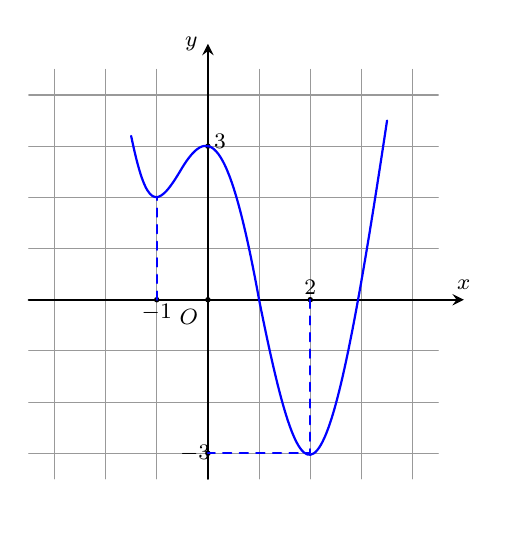
\begin{tikzpicture}[>=stealth,line join=round,line cap=round,font=\footnotesize,scale=0.65]
\draw[opacity=.4] (-3.5,-3.5)grid (4.5,4.5);
\draw[->,thick](-3.5,0)--(5,0)node[above]{$x$};
\draw[->,thick](0,-3.5)--(0,5)node[left]{$y$};
\foreach \point/\goc in {-1/-90,2/90}{
	\draw[fill=black](\point,0)circle(1.2pt)+(\goc:2.5mm)node[scale=1]{$\point$};}
\foreach \point/\goc in {3/20,-3/180}{
	\draw[fill=black](0,\point)circle(1.2pt)+(\goc:2.5mm)node[scale=1]{$\point$};}
	\draw[blue,thick]
	(-1.5,3.2)..controls(-1.2,1.75) and (-1,1.75) ..(-.55,2.5)..controls (0,3.45) and (0.4,3.3)..(1,0)..controls (1.9,-4.5) and (2.3,-4.5) .. (3.5,3.5);
\draw[fill=black] (0,0) circle (1.2pt)node[below left]{$O$};
\draw[dashed,blue,thick] (2,0)|-(0,-3) (-1,0)--(-1,2);
\end{tikzpicture}
}
\end{listEX}
\loigiai{
\begin{listEX}
\item Hàm số $y$ xác định $\Leftrightarrow \heva{& 1-x^2 \ne 0\\& -x \geq 0}$ $\Leftrightarrow \heva{& x \ne 1\\ & x \ne -1\\& x \leq 0}$ $\Leftrightarrow x \in (-\infty, 0] \setminus \{-1\}$.\\
Vậy $\mathscr{D}=(-\infty, 0] \setminus \{-1\}$.
\item Hàm số đồng biến trên $(-1;0)$ và $(2;+\infty)$.
\end{listEX}
}
\end{bt}

%%=====Bài 2
\begin{bt}%[0T3B2-2]%[tex đề HKI 22-23, Nguyễn Sĩ Đạt]
\begin{listEX}
\item  Xác định parabol $(P)\colon y=a x^2+b x+2$, biết rằng $(P)$ đi qua điểm $M(1 ; 5)$ và có trục đối xứng là đường thẳng $x=-\dfrac{1}{4}$. 
\item  Lập bảng biến thiên vẽ đồ thị hàm số $y=-2x^2+4x-3$.
\item 
\immini{
	Cổng của một công viên có khoảng trống phía trong cổng dạng parabol với chiều cao, độ rộng như hình vẽ. Cần đưa hàng hóa qua cổng này bằng xe tải có chiều cao là $5$ m và rộng $4$ m. Xe có qua được cổng không? Vì sao?
}{
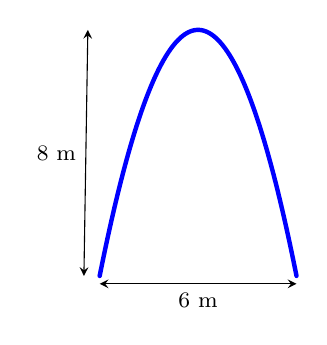
\begin{tikzpicture}[>=stealth,line join=round,line cap=round,font=\footnotesize,scale=.5]
	
	\tikzset{declare function ={x1=-3.5;x2=4.5;y1=-5.5;y2=-1.5;}}
	\tikzset{declare function={a=-1;b=2;c=-3; f(\x)=a*(\x)^2+b*(\x)+c;}}
	%	\clip (x1-1,y1-1)rectangle(x2+.5,y2+.5);
	
	\draw[samples=1000,domain=-1.5:3.5,ultra thick ,blue] plot(\x,{f(\x)});
	\draw[<->] (-1.5,{f(-1.5)-.2})--(3.5,{f(3.5)-.2})node[midway,below]{$6$ m};
	\draw[<->] (-1.8,{f(-b/(2*a))})--(-1.9,{f(3.5)})node[midway,left]{$8$ m};
	
\end{tikzpicture}	
}
\end{listEX}
\loigiai{
\begin{listEX}
\item  Vì $(P)$ đi qua điểm $M(1;5)$ nên $ 5=a+b+2 \Leftrightarrow a+b = 3$.\hfill (1)\\
Vì  $(P)$ có trục đối xứng là đường thẳng \begin{center}
	$x=-\dfrac{1}{4}$ nên  $- \dfrac{b}{2a} = -\dfrac{1}{4}  \Leftrightarrow 4b=2a \Leftrightarrow a-2b=0$.\hfill (2)
\end{center}
Từ (1) và (2), ta có hệ phương trình 
	 \begin{center}
	 	$\heva{& a+b=3\\& a-2b=0} \Leftrightarrow   \heva{& a=2\\& b=1.} $
	 \end{center} 
Vậy  $(P) \colon  y=2x^2+x+2$.
\item 
Hàm số $y=-2x^2+4x-3$.\\
Tập xác định: $\mathscr{D}=\mathbb{R}$.\\
Ta có $x_S=\dfrac{-b}{2a}=1 \Rightarrow y_S=-1$.\\
Suy ra $S(1;-1)$.
Do hàm số bậc hai có $a=-2<0$ nên ta có bảng biến thiên:
\begin{center}
	
\begin{tikzpicture}[>=stealth]
		\tkzTabInit[nocadre=false,lgt=1.5,espcl=3,deltacl=1]{$x$/1 ,$y$/2}
		{$-\infty$ , $1$ , $+\infty$}
		\tkzTabVar{-/$-\infty$ , +/$-1$ , -/$-\infty$}
	\end{tikzpicture}
\end{center}
Trong mặt phẳng tọa độ $Oxy$, đồ thị hàm số trên là một parabol $(P)$
\begin{itemize}
	\item Có đỉnh $S(1;-1)$.
	\item Có trục đối xứng là đường thẳng $x=1$.
	\item $a=-2<0$ bề lõm quay xuống.
	\item Cắt trục tung tại điểm có tung độ bằng $-3$, suy ra đồ thị đi qua điểm $A(0;-3)$. Điểm $(2;-3)$ đối xứng với điểm $(0;-3)$ qua trục đối xứng.
\end{itemize}

Ta có đồ thị hàm số như sau:
\begin{center}
	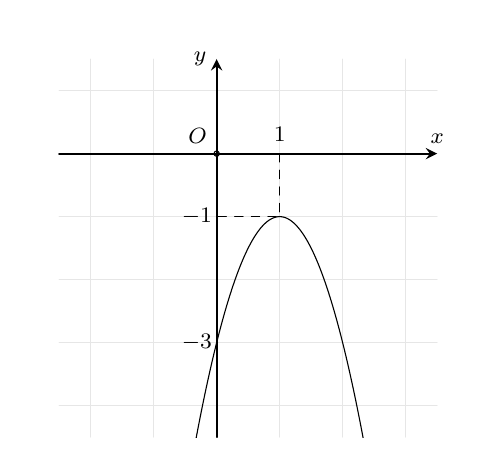
\begin{tikzpicture}[>=stealth,line join=round,line cap=round,font=\footnotesize,scale=.8]
		
		\tikzset{declare function ={x1=-2.5;x2=3.5;y1=-4.5;y2=1.5;}}
		\tikzset{declare function={a=-2;b=4;c=-3; f(\x)=a*(\x)^2+b*(\x)+c;}}
		\clip (x1-.5,y1)rectangle(x2+.5,y2+.5);
		\draw[opacity=.2,gray] (x1,y1)grid (x2,y2);
		\draw[->,thick](x1,0)--(x2,0)node[above]{$x$};
		\draw[->,thick](0,y1)--(0,y2)node[left]{$y$};
		\draw (0,0)circle(1.2pt)node[above left]{$O$};
		\draw[samples=1000,domain=-3.5:2.5] plot(\x,{f(\x)});
		\foreach \i/\goc in {1/90}{
			\draw (\i, 0) node[shift={(\goc:2.5mm)}]{$\i$};	
		}
		\foreach \i/\goc in {-1/180,-3/180}{
			\draw (0,\i) node[shift={(\goc:2.5mm)}]{$\i$};	
		}
		\draw[dashed] (1,0)|-(0,-1);
	\end{tikzpicture}
\end{center}
\item Xét hệ trục tọa độ $Oxy$ như hình vẽ.
\begin{center}
	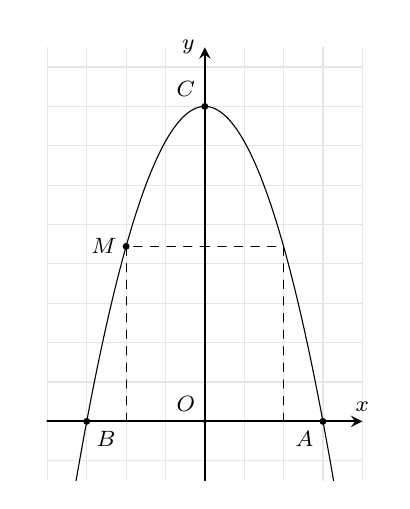
\begin{tikzpicture}[>=stealth,line join=round,line cap=round,font=\footnotesize,scale=.5]
		\coordinate[label=below left:$A$]     (A) at (3,0);
		\coordinate[label=below right:$B$] (B) at (-3,0);
		\coordinate[label=above left:$C$] (C) at (0,8);
		\coordinate[label=left:$M$] (M) at (-2,40/9);
		\tikzset{declare function ={x1=-4;x2=4;y1=-1.5;y2=9.5;}}
		\tikzset{declare function={a=-8/9;b=0;c=8; f(\x)=a*(\x)^2+b*(\x)+c;}}
		\clip (x1-.5,y1)rectangle(x2+.5,y2+.5);
		\draw[opacity=.2,gray] (x1,y1)grid (x2,y2);
		\draw[->,thick](x1,0)--(x2,0)node[above]{$x$};
		\draw[->,thick](0,y1)--(0,y2)node[left]{$y$};
		\draw (0,0)circle(1.2pt)node[above left]{$O$};
		\draw[samples=1000,domain=-3.5:3.5] plot(\x,{f(\x)});
		\foreach \diem in {A,B,C,M}	\fill[black] (\diem)circle(2.5pt);
		\draw[dashed] (-2,0)|-(0,40/9) (2,0)|-(0,40/9);
	\end{tikzpicture}
\end{center}
Cổng của công viên này có dạng parabol $(P)$. \\
Phương trình parabol này có dạng $(P)\colon y=ax^2+bx+c\,(a\neq 0)$.\\
Ta có $\heva{&A(3;0)\in (P)\\&B(-3;0)\in (P)\\&C(0;8)\in (P)}\Rightarrow \heva{&9a+3b+c=0\\&9a-3b+c=0\\&c=8}\Rightarrow \heva{&a=\dfrac{-8}{9}\\&b=0\\&c=8.}$\\
Do đó $(P)\colon y=\dfrac{-8}{9}x^2+8$.\\
Xét điểm $M(-2;y_M)\in (P)$, ta có $y_M=\dfrac{40}{9}<5$.\\
Do đó xe không thể đi qua cổng được.
\end{listEX}
}
\end{bt}

%%=====Bài 3
\begin{bt}%[0T2K2-2]%[tex đề HKI 22-23, Nguyễn Sĩ Đạt]
Người ta dự định dùng hai loại nguyên liệu để chiết xuất ít nhất $140$ kg chất A và $9$ kg chất B. Từ mỗi tấn nguyên liệu loại $I$ giá $4$ triệu đồng, có thể chiết xuất được $20 $ kg chất A và $0{,}6$ kg chất B. Từ mỗi tấn nguyên liệu loại II giá $3$ triệu đồng, có thể chiết xuất được $10$ kg chất A và $1{,}5$ kg chất $B$. Hỏi phải dùng bao nhiêu tấn nguyên liệu mỗi loại để chi phí mua nguyên liệu là ít nhất? Biết rằng cơ sở cung cấp nguyên liệu chỉ có thể cung cấp không quá $10$ tấn nguyên liệu loại I và không quá $9$ tấn nguyên liệu loại II.
\loigiai{
Gọi $x$, $y$ lần lượt là số tấn nguyên liệu loại I và loại II phải dùng.\\
Từ bài toán ta đưa được hệ bất phương trình
$\heva{&0 \leq x \leq 10\\&0 \leq y \leq 9\\&20x+10y\geq 140\\&0{,}6x+1{,}5y\geq 9.}\Leftrightarrow\heva{&0 \leq x \leq 10\\&0 \leq y \leq 9\\&2x+y\geq 14\\&2x+5y\geq 30.} (*)$\\
Biểu diễn miền nghiệm của hệ bất phương trình $(*)$ trên mặt phẳng tọa độ, ta được
\begin{center}
	\begin{tikzpicture}[scale=.6,font=\footnotesize  , line join=round, line cap=round, >=stealth,x=1cm,y=1cm]
		\def\xmin{-1}\def\xmax{16}\def\ymin{-1}\def\ymax{16}
		\draw[step=1,gray, very thin,opacity=0.2] (\xmin+0.1,\ymin+0.1) grid (\xmax-0.1,\ymax-0.1);
		\clip (\xmin+0.1,\ymin+0.1) rectangle (\xmax-0.1,\ymax-0.1);
		\draw[pattern = north east lines,opacity=.5,pattern color = red] plot[domain=\xmin:\xmax] (\x, {14-2*(\x)})--(-2,-2)--cycle;
		\draw[pattern = north west lines,opacity=.5,pattern color = green] plot[domain=\xmin:\xmax](\x, {6-0.4*(\x)})--(16,-2)--(-2,-2)--cycle;
		\draw[pattern = north east lines,opacity=.5,pattern color = violet] plot[domain=\xmin:\xmax] (-2,16)--(0,16)--(0,-1)--(-1,-1)--cycle
		(10,16)--(16,16)--(16,-1)--(10,-1)--cycle;
		\draw[pattern = north west lines,opacity=.5,pattern color = orange] (-1,0)--(16,0)--(16,-1)--(-1,-1)--cycle (-1,9)--(-1,16)--(16,16)--(16,9);
		\draw[line width=1,red,domain=\xmin:\xmax] plot (\x,{14-2*(\x)}) ;
		\draw[line width=1,green,domain=\xmin:\xmax] plot (\x,{6-0.4*(\x)}) ;
		\draw[line width=1,orange,domain=\xmin:\xmax] (-1,9)--(16,9) ;
		\draw[line width=1,violet,domain=\xmin:\xmax] (10,-1)--(10,16) ;
		\draw[line width=1.25,blue,->] (\xmin-0.1,0)--(\xmax-0.1,0) ;
		\draw[blue] (\xmax-0.25,-.1)node[below] {$x$};
		\draw[line width=1.25,blue,->] (0,\ymin-0.1)--(0,\ymax-0.1) ;
		\draw[blue](0,\ymax-0.25) node[left] {$y$};
		\draw[blue] (0,0) node [below left] {$O$};
		\foreach \x in {1,2,3,...,15}\draw[line width=0.75,blue] (\x,0.1)--(\x,-0.1) node [below] {$\x$};
		\foreach \y in {1,2,3,...,15}\draw[line width=0.75,blue] (0.1,\y)--(-0.1,\y) node [left] {$\y$};
		\fill[blue] (5,4)circle(1.5pt) node[above right]{$A$};
		\fill[blue] (10,2)circle(1.5pt) node[above left]{$B$};
		\fill[blue] (10,9)circle(1.5pt) node[below left]{$C$};
		\fill[blue] (2.5,9)circle(1.5pt) node[below right]{$D$};
	\end{tikzpicture}
\end{center}
Tổng chi phí là $f(x;y)=4x+3y$ (triệu đồng).\\
Ta tìm $x$, $y$ thỏa mãn hệ $(*)$ sao cho giá trị $f(x;y)$ nhỏ nhất.\\
Ta thấy miền nghiệm của hệ bất phương trình $(*)$ là miền tứ giác $ABCD$ nên $f(x;y)$ đạt giá trị nhỏ nhất tại các điểm $A(5;4)$, $B(10;2)$, $C(10;9)$, $D(2{,}5;9)$.\\
Ta có $f(5;4)=32$, $f(10;2)=46$, $f(10;9)=67$, $f(2{,}5;9)=37$.\\
Vậy $f(5;4)=32$ là giá trị nhỏ nhất của $f(x;y)$.\\
Vậy cần $5$ tấn nguyên liệu loại I và $4$ tấn nguyên liệu loại II để chi phí mua nguyên liệu là ít nhất là $32$ triệu.
}
\end{bt}


\begin{bt}%[0T5B2-5]%[Dự án đề kiểm tra HKI NH22-23- Mui Doan]%[Nguyễn Khuyến]
	\hfill
	\begin{enumerate}
		\item Cho hình chữa nhật $ABCD$ có $AB=2a$ và $AB=2BC$. Gọi $M$ là trung điểm $AD$. Tính theo $a$ các độ dài $\left\vert \overrightarrow{AB}+\overrightarrow{AD}\right\vert$ và $\left\vert \overrightarrow{MB}+\overrightarrow{MC}\right\vert$.
		\item Cho hình vuông $ABCD$ có cạnh bằng $5$. Tính tích vô hướng $ \overrightarrow{DA}\cdot\overrightarrow{BD}$.
		\item Cho tam giác $ABC$. Gọi $M$ là điểm trên cạnh $BC$ sao cho $MB=4MC$. Chứng minh $\overrightarrow{AM}=\dfrac{1}{5}\overrightarrow{AB}+\dfrac{4}{5}\overrightarrow{AC}$.
	\end{enumerate}
\loigiai{
	\begin{enumerate}
		\item 
		\immini{
	Vì $AB=2a$ nên $BC=a$.
	\begin{itemize}
		\item Ta có
	\allowdisplaybreaks
	\begin{eqnarray*}
		\left\vert \overrightarrow{AB}+\overrightarrow{AD}\right\vert&=&\left\vert \overrightarrow{AC}\right\vert
		\\
		&=&AC
		\\
		&=&\sqrt{AB^2+BC^2}
		\\
		&=&\sqrt{4a^2+a^2}
		\\
		&=&a\sqrt{5}.
	\end{eqnarray*}	
	\item Vẽ hình bình hành $MCNB$. Ta có
	\allowdisplaybreaks
	\begin{eqnarray*}
		\left\vert \overrightarrow{MB}+\overrightarrow{MC}\right\vert&=&\left\vert \overrightarrow{MN}\right\vert
		\\
		&=&MN
		\\
		&=&2MI~(\text{với}\,I\,\text{là trung điểm}\,BC, AD)
		\\
		&=&2AB
		\\
		&=&4a.
	\end{eqnarray*}	
\end{itemize}
	}
	{
	\begin{tikzpicture}
		\path (0,0) coordinate (A)++(2,0) coordinate (x)
		($(x)!-1!(A)$) coordinate (B)
		($ (B)!1!-90:(x)$) coordinate (C)
		 ($(A)!1!90:(x)$) coordinate (D)
		 ($(A)!.5!(D)$) coordinate (M)
		 ($(B)+(C)-(M)$) coordinate (N)
		 ($(B)!.5!(C)$) coordinate (I)
		 ;
		\draw (B)--(C)--(D)--(A)--cycle (A)--(C) (M)--(C)--(N)--(B)--cycle (M)--(N);
		\foreach \t/\g in {A/180,B/-90,C/90,D/180,M/180,N/0,I/-60}{
			\draw[fill=black] (\t) circle (1pt) node[shift={(\g:7pt)},font=\scriptsize]{$ \t $};
		}
	\end{tikzpicture}
		}
		\item Ta có
		\immini{
		\allowdisplaybreaks
		\begin{eqnarray*}
			 \overrightarrow{DA}\cdot\overrightarrow{BD}&=&-\overrightarrow{DA}\cdot\overrightarrow{DB}
			 \\
			 &=&-DA\cdot DB\cdot \cos \left(\overrightarrow{DA},\overrightarrow{DB}\right)
			 \\
			 &=&-5\cdot 5\sqrt{2}\cdot \cos 45^\circ
			 \\
			 &=&-5\cdot 5\sqrt{2}\cdot \dfrac{\sqrt{2}}{2}
			 \\
			 &=&-25.
		 \end{eqnarray*}
		}
		{
		\begin{tikzpicture}
			\path (0,0) coordinate (A)
			(2,0) coordinate (B)
			($ (B)!1!-90:(A)$) coordinate (C)
			($(A)!1!90:(B)$) coordinate (D)
			;
			\draw (B)--(C)--(D)--(A)--cycle (D)--(B) ;
			\foreach \t/\g in {A/180,B/0,C/0,D/180}{
				\draw[fill=black] (\t) circle (1pt) node[shift={(\g:7pt)},font=\scriptsize]{$ \t $};
			}
		\end{tikzpicture}
		}
		\item Do $M$ là điểm trên cạnh $BC$ và $MB=4MC$ suy ra
		\allowdisplaybreaks
		\begin{eqnarray*}
			&&\overrightarrow{MB}=-4\overrightarrow{MC}
			\\
			&\Leftrightarrow&\overrightarrow{MA}+\overrightarrow{AB}=-4\left(\overrightarrow{MA}+\overrightarrow{AC}\right)
			\\
			&\Leftrightarrow&-\overrightarrow{AM}+\overrightarrow{AB}=4\overrightarrow{AM}-4\overrightarrow{AC}
			\\
			&\Leftrightarrow&5\overrightarrow{AM}=\overrightarrow{AB}+4\overrightarrow{AC}
			\\
			&\Leftrightarrow&\overrightarrow{AM}=\dfrac{1}{5}\overrightarrow{AB}+\dfrac{4}{5}\overrightarrow{AC}.
		\end{eqnarray*}
	\end{enumerate}
}
\end{bt}
%Bài 5
\begin{bt}%[0T5K3-5]%[Dự án đề kiểm tra HKI NH22-23- Mui Doan]%[Nguyễn Khuyến]
	Cho tam giác $ABC$. Gọi $P$, $Q$, $R$ thỏa hệ thức $3\overrightarrow{PB}+4\overrightarrow{PC}=\overrightarrow{0}$, $2\overrightarrow{RA}+\overrightarrow{RB}=\overrightarrow{0}$, $3\overrightarrow{QA}-2\overrightarrow{QC}=\overrightarrow{0}$. Chứng minh $P$, $Q$, $R $ thẳng hàng.
	\loigiai{
	\begin{itemize}
		\item Ta có
		\allowdisplaybreaks
		\begin{eqnarray*}
			&&3\overrightarrow{PB}+4\overrightarrow{PC}=\overrightarrow{0}
			\\
			&\Leftrightarrow& 3\left(\overrightarrow{PA}+\overrightarrow{AB}\right)+4\left(\overrightarrow{PA}+\overrightarrow{AC}\right)=\overrightarrow{0}
			\\
			&\Leftrightarrow& 7\overrightarrow{PA}+3\overrightarrow{AB}+4\overrightarrow{AC}=\overrightarrow{0}
			\\
			&\Leftrightarrow&
			-7\overrightarrow{AP}+3\overrightarrow{AB}+4\overrightarrow{AC}=\overrightarrow{0}
			\\
			&\Leftrightarrow&
			\overrightarrow{AP}=\dfrac{3}{7}\overrightarrow{AB}+\dfrac{4}{7}\overrightarrow{AC}.
		\end{eqnarray*}
	\item Ta có
	\allowdisplaybreaks
	\begin{eqnarray*}
		&&2\overrightarrow{RA}+\overrightarrow{RB}=\overrightarrow{0}
		\\
		&\Leftrightarrow& 2\overrightarrow{RA}+\overrightarrow{RA}+\overrightarrow{AB}=\overrightarrow{0}
		\\
		&\Leftrightarrow& -3\overrightarrow{AR}+\overrightarrow{AB}=\overrightarrow{0}
		\\
		&\Leftrightarrow&
		3\overrightarrow{AR}=\overrightarrow{AB}
		\\
		&\Leftrightarrow&
		\overrightarrow{AR}=\dfrac{1}{3}\overrightarrow{AB}.
	\end{eqnarray*}
	\item Ta có
	\allowdisplaybreaks
	\begin{eqnarray*}
		&&3\overrightarrow{QA}-2\overrightarrow{QC}=\overrightarrow{0}
		\\
		&\Leftrightarrow& 3\overrightarrow{QA}-2\left(\overrightarrow{QA}+\overrightarrow{AC}\right)=\overrightarrow{0}
		\\
		&\Leftrightarrow& \overrightarrow{QA}-2\overrightarrow{AC}=\overrightarrow{0}
		\\
		&\Leftrightarrow&
		-\overrightarrow{AQ}-2\overrightarrow{AC}=\overrightarrow{0}
		\\
		&\Leftrightarrow&
		\overrightarrow{AQ}=-2\overrightarrow{AC}.
	\end{eqnarray*}
	\end{itemize}	
	Ta có 
	\allowdisplaybreaks
	\begin{eqnarray*}
		\overrightarrow{PQ}&=&\overrightarrow{PA}+\overrightarrow{AQ}
		\\
		&=&-\overrightarrow{AP}+\overrightarrow{AQ}
		\\
		&=&-\left(\dfrac{3}{7}\overrightarrow{AB}+\dfrac{4}{7}\overrightarrow{AC}\right)-2\overrightarrow{AC}
		\\
		&=&-\dfrac{3}{7}\overrightarrow{AB}-\dfrac{18}{7}\overrightarrow{AC}. \qquad(1)
	\end{eqnarray*}
	\allowdisplaybreaks
	\begin{eqnarray*}
		\overrightarrow{PR}&=&\overrightarrow{PA}+\overrightarrow{AR}
		\\
		&=&-\overrightarrow{AP}+\overrightarrow{AR}
		\\
		&=&-\left(\dfrac{3}{7}\overrightarrow{AB}+\dfrac{4}{7}\overrightarrow{AC}\right)+\dfrac{1}{3}\overrightarrow{AB}
		\\
		&=&-\dfrac{2}{21}\overrightarrow{AB}-\dfrac{4}{7}\overrightarrow{AC}. \qquad(2)
	\end{eqnarray*}
	Từ $(1)$ và $(2)$ suy ra $\overrightarrow{PQ}=\dfrac{9}{2}\vv{PR}$ suy ra $\overrightarrow{PQ}, \overrightarrow{PR}$ cùng phương.\\
	Vậy $P$, $Q$, $R $ thẳng hàng.
	}
\end{bt}
